\chapter{指定参考点或坐标系}
Tikz 默认单位是厘米,直角坐标下,二元数 (1,2) 表示 $x$ 方向一倍的单位长度 (1cm) ,$y$方向2倍的单位长度 (1cm) 。这种表示是绝对坐标。当然最好是添加上单位。比如(1cm,2pt), 表示$x$ 方向 1cm,$y$ 方向2个磅\footnote{磅,pt 是 point的简写,是英文字号的单位,在欧美字体度量系统常用, 1pt 大约为 0.35 毫米。常用的 5 号字体是 10.5 磅,绝对长度约 3.7 毫米。} 长度。其用法如下:
\begin{verbatim}
(xpt,ycm): xpt in x-direction and ycm in y-directions.
(xdegree:ycm): ycm in direction x degree.
+(x,y): xcm above and ycm right from the previous specified position.
++(x,y): xcm above and ycm right from the previous specified position 
and making this the new specified position.
(x1,y1) -- (x2,y2): straight line from (x1,y1) to (x2,y2);
(x1,y1) -| (x2,y2): a horizontal and vertical line from (x1,y1) to (x2,y2);
(x1,y1) |- (x2,y2); a vertical and horizontal line from (x1,y1) to (x2,y2);
\end{verbatim}
\begin{lstlisting}
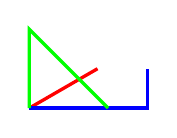
\begin{tikzpicture}
\draw[red,very thick] (30:1cm) -- (0,0);
\draw[blue,very thick] (0,0) -| +(1.5,0.5) ;
\draw[green,very thick] (0,0) |- ++(0,1) -- (1,0);
\end{tikzpicture}
\end{lstlisting}
\begin{center}
	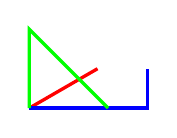
\begin{tikzpicture}
	\draw[red,very thick] (30:1cm) -- (0,0);
	\draw[blue,very thick] (0,0) -| +(1.5,0.5) ;
	\draw[green,very thick] (0,0) |- ++(0,1) -- (1,0);
	\end{tikzpicture}
\end{center}
另一种方式的坐标是参考上一个点的参考坐标系,通常在二元数前添
加“ + ”号进行标识。比如 +(0cm, 1cm) 表示相对上一个点向上移动 1cm。而 ++(2cm,0cm) 表示,相对于上一个点向右移动 2cm。下面给出几个例子体会 + 与 ++ 的区别。

在极坐标系下, 使用类似 (30:1cm) 的方式, 表示 30 度方向的一个 1cm长度所在那个点。
\begin{tikzpicture}[>=Stealth,scale=0.2,smooth]
\draw[->](-10,0)--(0,0) node[below left=-1.2pt]{$O$}--(20,0) node[below=1.5pt]{$x$};
\draw[->](0,-8)--(0,10)node[left]{$y$};
\draw (0,0) sin (3,3) cos (6,0);
\draw (6,0) sin (9,-3) cos (12,0);
\end{tikzpicture}
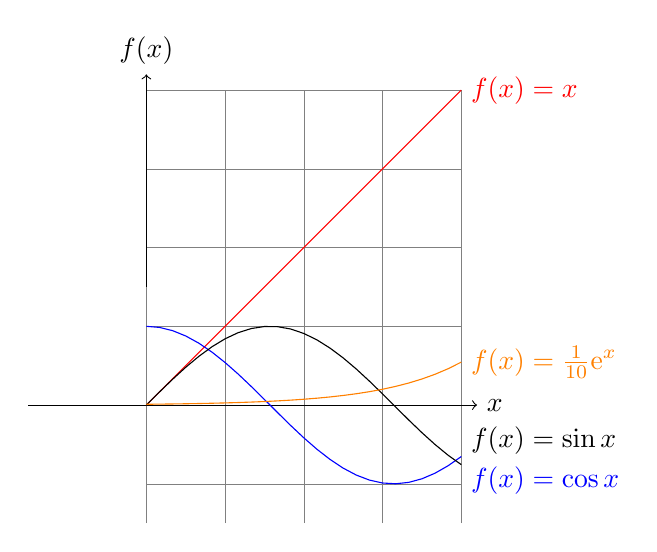
\begin{tikzpicture}[domain=0:4]
\draw[very thin,color=gray] (0,-1.5) grid (4.0,4.0);
\draw[->] (-1.5,0) -- (4.2,0) node[right] {$x$};
\draw[->] (0,1.5) -- (0,4.2) node[above] {$f(x)$};
\draw[color=red] plot (\x,\x) node[right] {$f(x) =x$};
\draw[color=blue] plot (\x,{cos(\x r)}) node[below right] {$f(x) = \cos x$};
\draw[black] plot (\x,{sin(\x r)}) node[above right] {$f(x) = \sin x$};
\draw[color=orange] plot (\x,{0.01*exp(\x)})
node[right] {$f(x) = \frac{1}{10} \mathrm e^x$};
\end{tikzpicture}
\begin{tikzpicture}[x={(-.1cm,-.15cm)},y={(1cm,0cm)},z={(0cm,1cm)}]
\draw[->] (0,0,0) -- (10,0,0) node[below] {$x$};
\draw[->] (0,-2,0) -- (0,2,0) node[right] {$y$};
\draw[->] (0,0,-2) -- (0,0,3) node[above] {$z$};
\draw[color=red] plot[domain=0:2*pi] ({sin(\x r)},{cos(\x r)},2);
\draw[color=red] (0,0,0) -- (0,1,2) (0,0,0) -- (0,-1,2);
\end{tikzpicture}

\begin{tikzpicture}
\draw(0,0)coordinate(A)node[left]{$A$}(2,0)coordinate(B)node[below]{$B$}
(1.5,0.6)coordinate(D)node[left]{$D$}(3.5,0.6)coordinate(C)node[right]{$C$};
\draw(0,4)coordinate(A1)node[left]{$A_1$}(2,4)coordinate(B1)node[below right=-2pt and -2pt]{$B_1$}
(1.5,4.6)coordinate(D1)node[above]{$D_1$}(3.5,4.6)coordinate(C1)node[right]{$C_1$};
\draw(A)--(A1)--(D1)--(C1)--(B1)--(A1)(A)--(B)--(C)--(C1)(B)--(B1);
\draw(0.75,2.3)coordinate(N)node[left]{$N$}
(2,2)coordinate(M)node[left]{$M$}(2.75,0.3)coordinate(E)node[right]{$E$};
\draw[densely dashed](A)--(D)--(A1)(D1)--(D)--(C1)(D)--(C)(N)--(M)(D)--(E);
\draw(C1)--(E)(A1)--(M)--(A);
\end{tikzpicture}
\begin{tikzpicture}
\draw(-0.3,0.3)coordinate(A)node[left]{$A$}--(0,0)coordinate(B)node[below]{$B$}--(1.8,0)coordinate(C)node[below]{$C$};
\draw[densely dashed](A)--(C);
\draw[shift={(1cm,1.732cm)}](-0.3,0.3)coordinate(D)node[left]{$D$}--(0,0)coordinate(E)node[below right=0pt and -4pt]{$E(F)$}--(1.8,0)coordinate(G)node[right]{$G$}--(D);
\draw(A)--(D)(B)--(E)(C)--(G);
\end{tikzpicture}
\begin{tikzpicture}[>=Stealth]
\draw(-0.3,0.3)coordinate(A)node[left]{$A$}--(0,0)coordinate(B)node[below]{$B$}--(1.8,0)coordinate(C)node[below]{$C$};
\draw[densely dashed](A)--(C);
\draw[shift={(1cm,1.732cm)}](-0.3,0.3)coordinate(D)node[left]{$D$}--(0,0)coordinate(E)node[below right=0pt and -4pt]{$E(F)$}--(1.8,0)coordinate(G)node[right]{$G$}--(D);
\draw(A)--(D)(B)--(E)(C)--(G);
\draw[->](1,0)node[below]{$H$}--(3.2,0)node[below]{$x$};
\draw[->](1,0)--(1,2.7)node[left]{$z$};
\draw[->,densely dashed](1,0)--(0.18,0.8)node[below]{$y$};
\end{tikzpicture}

\begin{tikzpicture}[scale=0.7]
\draw(0,0)coordinate(A)node[left]{$A$}(6,0)coordinate(B)node[right]{$B$}
(2,2.4)coordinate(D)node[left]{$D$}(8,2.4)coordinate(C)node[right]{$C$}
(0,3.6)coordinate(A1)node[left]{$A_1$}(2,6)coordinate(D1)node[above]{$D_1$}
(8,6)coordinate(C1)node[above]{$C_1$}(4,3)coordinate(O)node[left]{$O$}
(6,3.6)coordinate(B1)node[below left=-0.5pt and -4pt]{$B_1$}(7.1,1.32)coordinate(E)node[right]{$E$}
(6,1.8)coordinate(H)node[left]{$H$}(7,4.8)coordinate(G)node[left]{$G$}
(8,4.2)coordinate(F)node[right]{$F$};
\draw(A)--(A1)--(D1)--(C1)--(B1)--(A1)(A)--(B)--(B1)(B)--(C)--(C1)
(E)--(F)--(G)--(H)--(E);
\draw[densely dashed](A)--(D)--(D1)(D)--(C)(H)--(O)--(E)(F)--(O)--(G);
\end{tikzpicture}
\begin{tikzpicture}
\draw(0,0)coordinate(E)node[below]{$E$}--++(0,1)coordinate(D)node[above]{$D$}--++(2,0)coordinate(A)node[above]{$A$}--++(0,-1)coordinate(B)node[below left=0pt and -2pt]{$B$}--(E)
(B)--++(2,0)coordinate(C)node[above right=-2pt and -3pt]{$C$}--++(-60:2)coordinate(G)node[below]{$G$}
--++(-2,0)coordinate(F)node[below]{$F$}--(B)(A)--(C);
\end{tikzpicture}